\documentclass[tikz]{standalone}

\begin{document}
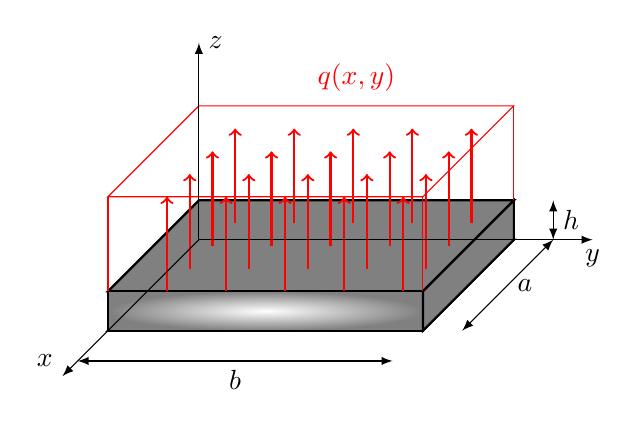
\begin{tikzpicture}
	\def\h{.5}
	\def\a{3}
	\def\b{4}
	\def\q{1.2}
	
	\draw[thick] (0,0,0) -- (\b,0,0) -- (\b,0,\a) -- (0,0,\a) -- cycle; % Cara inferior
	\draw[thick, fill=gray] (0,\h,0) -- (\b,\h,0) -- (\b,\h,\a) -- (0,\h,\a) -- cycle; % Cara superior
	\draw[thick, outer color=gray, inner color=white] (0,0,\a) rectangle (\b, \h, \a) ; % Cara frontal
	\draw[thick, fill=gray] (\b,0,0) -- (\b,0,\a) -- (\b, \h, \a) -- (\b,\h, 0) -- cycle; % Cara derecha
	
	% Etiquetas de dimensiones
	\draw[latex-latex] (\b + \h,0,0) -- (\b + \h,\h,0) node[midway,right] {$h$}; 
	\draw[latex-latex] (0,0,\a + 2*\h) -- (\b,0,\a + 2*\h) node[midway,below] {$b$};
	\draw[latex-latex] (\b + \h,0,0) -- (\b + \h,0,\a) node[midway,right] {$a$};
	
	% Carga distribuida
	\foreach \x in {.75,1.5,...,\b} {
		\foreach \z in {0.75,1.5,...,\a} {
			\draw[->, red, thick] (\x,\h,\z) -- (\x,\h+\q,\z); 
		}
	}
	\node[red] at (\b/2,\h+1.3*\q,0) {$q(x, y)$};
	
	\draw[red] (0, \h+\q, 0) -- (\b, \h + \q, 0) -- (\b, \h + \q, \a) -- (0, \h + \q, \a) -- cycle; % cara superior de la carga
	\draw[red] (\b, \h, 0) -- (\b, \h+\q, 0);  % Arista posterior derecha
	\draw[red] (\b, \h, \a) -- (\b, \h+\q, \a);  % Arista frontal derecha
	\draw[red] (0, \h, \a) -- (0, \h+\q, \a);  % Arista frontal izquierda
	
	% Sistema de coordenadas
	\draw[-latex] (0,0,0) -- (5,0,0) node[below] {$y$};
	\draw[-latex] (0,0,0) -- (0,2.5,0) node[right] {$z$};
	\draw[-latex] (0,0,0) -- (0,0,4.5) node[above left] {$x$};
\end{tikzpicture}
\end{document}